% -*- coding: utf-8 -*-
%-------------------------designed by zcf--------------
\documentclass[UTF8,a4paper,10pt]{ctexart}
\usepackage[left=3.17cm, right=3.17cm, top=2.74cm, bottom=2.74cm]{geometry}
\usepackage{amsmath}
\usepackage{graphicx,subfig}
\usepackage{float}
\usepackage{cite}
\usepackage{caption}
\usepackage{enumerate}
\usepackage{booktabs} %表格
\usepackage{multirow}
\newcommand{\tabincell}[2]{\begin{tabular}{@{}#1@{}}#2\end{tabular}}  %表格强制换行
%-------------------------字体设置--------------
% \usepackage{times} 
\usepackage{ctex}
\setCJKmainfont[ItalicFont=Noto Sans CJK SC Bold, BoldFont=Noto Serif CJK SC Black]{Noto Serif CJK SC}
\newcommand{\yihao}{\fontsize{26pt}{36pt}\selectfont}           % 一号, 1.4 倍行距
\newcommand{\erhao}{\fontsize{22pt}{28pt}\selectfont}          % 二号, 1.25倍行距
\newcommand{\xiaoer}{\fontsize{18pt}{18pt}\selectfont}          % 小二, 单倍行距
\newcommand{\sanhao}{\fontsize{16pt}{24pt}\selectfont}  %三号字
\newcommand{\xiaosan}{\fontsize{15pt}{22pt}\selectfont}        % 小三, 1.5倍行距
\newcommand{\sihao}{\fontsize{14pt}{21pt}\selectfont}            % 四号, 1.5 倍行距
\newcommand{\banxiaosi}{\fontsize{13pt}{19.5pt}\selectfont}    % 半小四, 1.5倍行距
\newcommand{\xiaosi}{\fontsize{12pt}{18pt}\selectfont}            % 小四, 1.5倍行距
\newcommand{\dawuhao}{\fontsize{11pt}{11pt}\selectfont}       % 大五号, 单倍行距
\newcommand{\wuhao}{\fontsize{10.5pt}{15.75pt}\selectfont}    % 五号, 单倍行距
%-------------------------章节名----------------
\usepackage{ctexcap} 
\CTEXsetup[name={,、},number={ \chinese{section}}]{section}
\CTEXsetup[name={(,)},number={\chinese{subsection}}]{subsection}
\CTEXsetup[name={,.},number={\arabic{subsubsection}}]{subsubsection}
%-------------------------页眉页脚--------------
\usepackage{fancyhdr}
\pagestyle{fancy}
\lhead{\kaishu \leftmark}
% \chead{}
\rhead{\kaishu 计算机网络第一次实验}%加粗\bfseries 
\lfoot{}
\cfoot{\thepage}
\rfoot{}
\renewcommand{\headrulewidth}{0.1pt}  
\renewcommand{\footrulewidth}{0pt}%去掉横线
\newcommand{\HRule}{\rule{\linewidth}{0.5mm}}%标题横线
\newcommand{\HRulegrossa}{\rule{\linewidth}{1.2mm}}
%-----------------------伪代码------------------
\usepackage{algorithm}  
\usepackage{algorithmicx}  
\usepackage{algpseudocode}  
\floatname{algorithm}{Algorithm}  
\renewcommand{\algorithmicrequire}{\textbf{Input:}}  
\renewcommand{\algorithmicensure}{\textbf{Output:}} 
\usepackage{lipsum}  
\makeatletter
\newenvironment{breakablealgorithm}
  {% \begin{breakablealgorithm}
  \begin{center}
     \refstepcounter{algorithm}% New algorithm
     \hrule height.8pt depth0pt \kern2pt% \@fs@pre for \@fs@ruled
     \renewcommand{\caption}[2][\relax]{% Make a new \caption
      {\raggedright\textbf{\ALG@name~\thealgorithm} ##2\par}%
      \ifx\relax##1\relax % #1 is \relax
         \addcontentsline{loa}{algorithm}{\protect\numberline{\thealgorithm}##2}%
      \else % #1 is not \relax
         \addcontentsline{loa}{algorithm}{\protect\numberline{\thealgorithm}##1}%
      \fi
      \kern2pt\hrule\kern2pt
     }
  }{% \end{breakablealgorithm}
     \kern2pt\hrule\relax% \@fs@post for \@fs@ruled
  \end{center}
  }
\makeatother
%------------------------代码-------------------
\usepackage{xcolor} 
\usepackage{listings} 
\lstset{ 
breaklines,%自动换行
basicstyle=\small,
escapeinside=``,
keywordstyle=\color{ blue!70} \bfseries,
commentstyle=\color{red!50!green!50!blue!50},% 
stringstyle=\ttfamily,% 
extendedchars=false,% 
linewidth=\textwidth,% 
numbers=left,% 
numberstyle=\tiny \color{blue!50},% 
frame=trbl% 
rulesepcolor= \color{ red!20!green!20!blue!20} 
}
%------------超链接----------
\usepackage[colorlinks,linkcolor=black,anchorcolor=blue]{hyperref}
%------------------------TODO-------------------
\usepackage{enumitem,amssymb}
\newlist{todolist}{itemize}{2}
\setlist[todolist]{label=$\square$}
% for check symbol 
\usepackage{pifont}
\newcommand{\cmark}{\ding{51}}%
\newcommand{\xmark}{\ding{55}}%
\newcommand{\done}{\rlap{$\square$}{\raisebox{2pt}{\large\hspace{1pt}\cmark}}\hspace{-2.5pt}}
\newcommand{\wontfix}{\rlap{$\square$}{\large\hspace{1pt}\xmark}}
%------------------------水印-------------------
\usepackage{tikz}
\usepackage{xcolor}
\usepackage{eso-pic}

\newcommand{\watermark}[3]{\AddToShipoutPictureBG{
\parbox[b][\paperheight]{\paperwidth}{
\vfill%
\centering%
\tikz[remember picture, overlay]%
  \node [rotate = #1, scale = #2] at (current page.center)%
    {\textcolor{gray!80!cyan!30!magenta!30}{#3}};
\vfill}}}



%———————————————————————————————————————————正文———————————————————————————————————————————————
%----------------------------------------------
\begin{document}
\begin{titlepage}
    \begin{center}
    
\includegraphics[width=0.8\textwidth]{NKU.png}\\[1cm]    
    \textsc{\Huge \kaishu{\textbf{南\ \ \ \ \ \ 开\ \ \ \ \ \ 大\ \ \ \ \ \ 学}} }\\[0.9cm]
    \textsc{\huge \kaishu{\textbf{网\ \ 络\ \ 空\ \ 间\ \ 安\ \ 全\ \ 学\ \ 院}}}\\[0.5cm]
    \textsc{\Large \textbf{计算机网络实验3-4}}\\[0.8cm]
    \HRule \\[0.9cm]
    { \LARGE \bfseries 基于UDP服务设计可靠传输协议并编程实现(性能对比测试)}\\[0.4cm]
    \HRule \\[2.0cm]
    \centering
    \textsc{\LARGE 马世骐\ \ 6016252\kaishu{\ \ \ \ }}\\[0.5cm]
    \textsc{\LARGE \kaishu{年级\ :\ 2020级}}\\[0.5cm]
    \textsc{\LARGE \kaishu{专业\ :\ 经济伯苓班}}\\[0.5cm]
    \textsc{\LARGE \kaishu{指导教师\ :\ 张建忠、徐敬东}}\\[0.5cm]
    \vfill
    {\Large \today}
    \end{center}
\end{titlepage}
%-------------摘------要--------------
\newpage
\thispagestyle{empty}
%----------------------------------------------------------------
\tableofcontents
%----------------------------------------------------------------
\newpage
\watermark{60}{10}{NKU}
\setcounter{page}{1}
%----------------------------------------------------------------
\section{实验基本描述}
%——————————————————————————————————————
基于给定的实验测试环境,通过改变延迟时间和丢包率,完成下面3组性能对比实验:
\begin{enumerate}
  \item 停等机制与滑动窗口机制性能对比
  \item 滑动窗口机制中不同窗口大小对性能的影响
  \item 有拥塞控制和无拥塞控制的性能比较
\end{enumerate}

%----------------------------------------------------------------
\section{实验具体工作}
%——————————————————————————————————————
\subsection{实验设计}
本次实验的数据都是经过三次测试之后取的平均值。\par
表格中的内容为吞吐率大小,单位Kbps\par
严格控制变量,每次只会改变同一个变量,保持其它变量不变。
\subsection{停等机制与滑动窗口机制性能对比}
\subsubsection{改变丢包率}
延时设为0,得到结果如下所示:
表
\begin{table}[!htbp]
  \centering
  \begin{tabular}{ccccccccccc}
  \toprule  
  机制$\backslash$丢包率& 0\%& 2\%& 5\%& 10\%\\
  \midrule
  停等& 960.825& 864.332& 550.20& 105.227\\
  滑动窗口(GBN)& 1644.26& 1075.429& 569.467& 154.318\\
  \bottomrule
  \end{tabular}
  \caption{性能测试吞吐率结果(单位:Kbps)}
\end{table}

关于传输时间,由于使用路由程序转发本身就会带来一定的延时,因此这里的数据并不能真实反映程序性能。
\begin{table}[!htbp]
  \centering
  \begin{tabular}{ccccccccccc}
  \toprule  
  机制$\backslash$丢包率& 0\%& 2\%& 5\%& 10\%\\
  \midrule
  停等& 23.435& 36.651& 109.989& 285.213\\
  滑动窗口(GBN)& 6.391& 22.623& 72.374& 179.651\\
  \bottomrule
  \end{tabular}
  \caption{性能测试延时结果(单位:S)}
\end{table}

绘制曲线如下所示:
\begin{figure}[H]
    \centering
    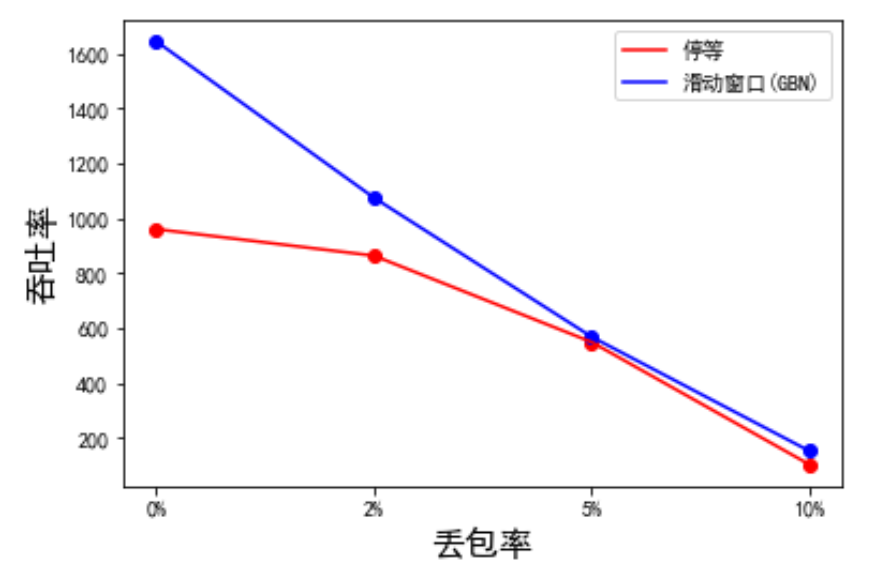
\includegraphics[scale=0.6]{计网1.png}
    \label{fig:1}
\end{figure}
\begin{figure}[H]
    \centering
    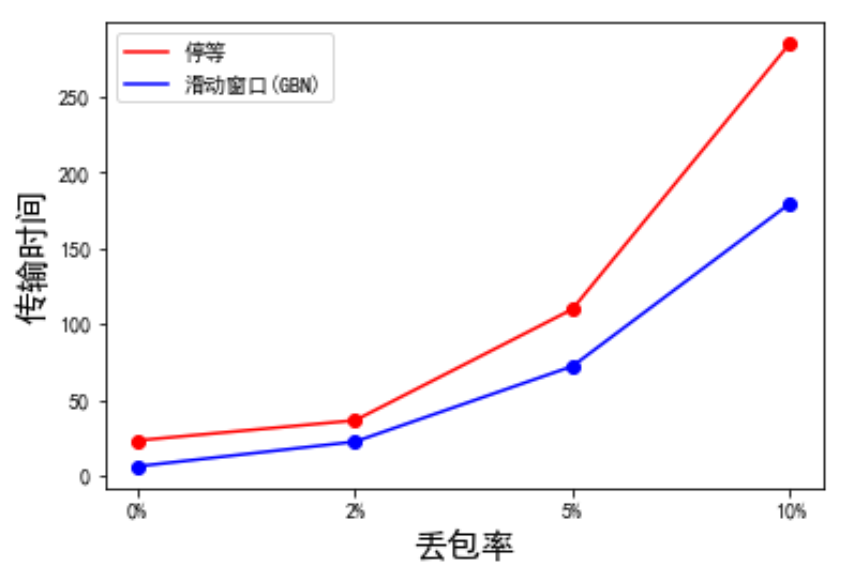
\includegraphics[scale=0.6]{计网2.png}
    \label{fig:2}
\end{figure}
\subsubsection{改变延时}
延时单位为ms。丢包设为0,得到结果如下所示:
表
\begin{table}[!htbp]
  \centering
  \begin{tabular}{ccccccccccc}
  \toprule  
  机制$\backslash$延时& 0s& 20s& 50s& 100s\\
  \midrule
  停等& 960.825& 560.576& 250.119& 44.291\\
  滑动窗口(GBN)& 1644.26& 762.343& 312.856& 65.786\\
  \bottomrule
  \end{tabular}
  \caption{性能测试吞吐率结果(单位:Kbps)}
\end{table}

关于传输时间,由于使用路由程序转发本身就会带来一定的延时,因此这里的数据并不能真实反映程序性能。延时单位为ms。
\begin{table}[!htbp]
  \centering
  \begin{tabular}{ccccccccccc}
  \toprule  
  机制$\backslash$延时& 0s& 20s& 50s& 100s\\
  \midrule
  停等& 23.435& 62.196& 131.482& 432.477\\
  滑动窗口(GBN)& 6.391& 50.026& 120.561& 365.21\\
  \bottomrule
  \end{tabular}
  \caption{性能测试延时结果(单位:S)}
\end{table}

绘制曲线如下所示:
\begin{figure}[H]
    \centering
    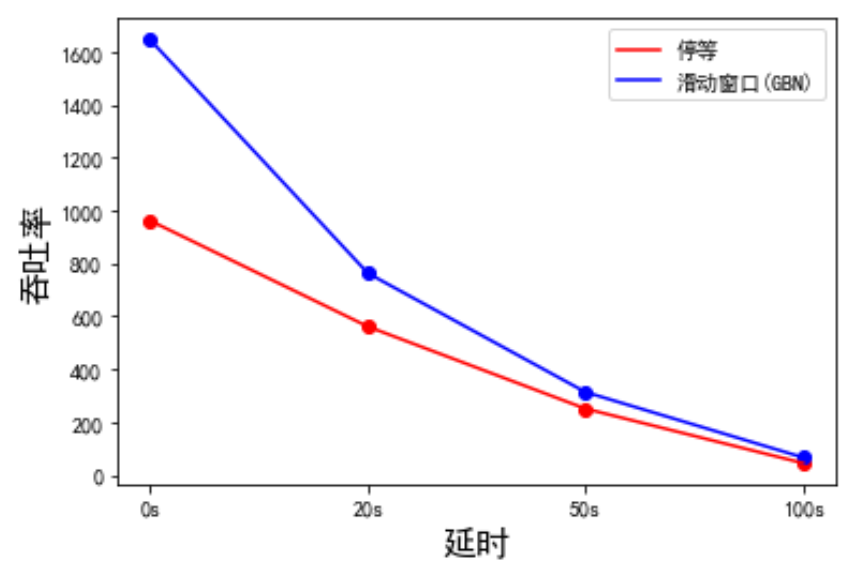
\includegraphics[scale=0.6]{计网3.png}
    \label{fig:3}
\end{figure}
\begin{figure}[H]
    \centering
    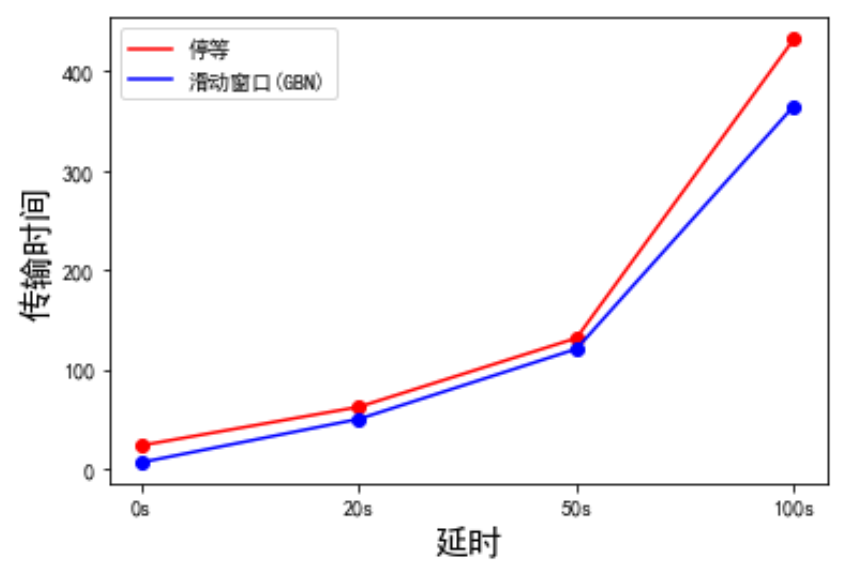
\includegraphics[scale=0.6]{计网4.png}
    \label{fig:4}
\end{figure}
\subsubsection{结果分析}
总体来说:
大体上滑动窗口机制比停等机制的效率更高,因为滑动窗口机制允许发送多条消息,大大优化了停等机制中每发一个报都要等一个ACK的情况,同时等待对方回复的ACK,减少RTT的影响\par
在有延时的情况下,GBN表现更好,原因同上,停等机制需要每条消息单独等待时延和RTT,而窗口可以同时等待多条\par
丢包率大时GBN效率比停低,使用滑动窗口机制相对于停等机制的加速比明显降低,甚至有的时候性能不如停等机制。这是由于滑动窗口在丢包时需要重传数据包并等待重传数据包的ACK收到之后才能将窗口移动,因此定长滑动窗口受丢包率的影响较大
\subsection{滑动窗口机制中不同窗口大小对性能的影响}
\subsubsection{改变丢包率}
延时设为0,得到结果如下所示:
表
\begin{table}[!htbp]
  \centering
  \begin{tabular}{ccccccccccc}
  \toprule  
  窗口大小$\backslash$丢包率& 0\%& 2\%& 5\%& 10\%\\
  \midrule
  6& 1022.322& 264.897& 168.695& 90.6781\\
  10(GBN)& 1044.26& 343.323& 198.482& 69.5384\\
  \bottomrule
  \end{tabular}
  \caption{性能测试吞吐率结果(单位:Kbps)}
\end{table}

关于传输时间,由于使用路由程序转发本身就会带来一定的延时,因此这里的数据并不能真实反映程序性能。
\begin{table}[!htbp]
  \centering
  \begin{tabular}{ccccccccccc}
  \toprule  
  窗口大小$\backslash$丢包率& 0\%& 2\%& 5\%& 10\%\\
  \midrule
  6& 6.842& 103.376& 196.746& 466.892\\
  10& 6.391& 99.998& 175.886& 379.265\\
  \bottomrule
  \end{tabular}
  \caption{性能测试延时结果(单位:S)}
\end{table}

绘制曲线如下所示:
\begin{figure}[H]
    \centering
    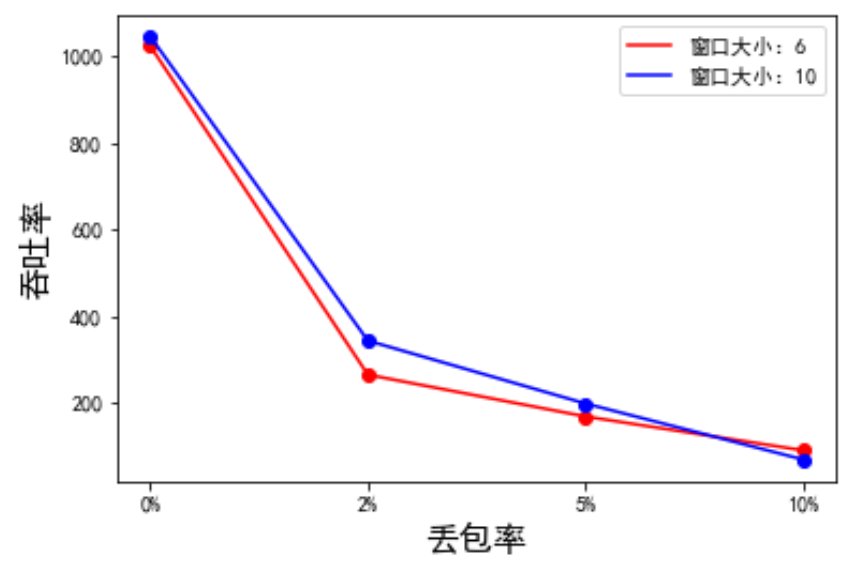
\includegraphics[scale=0.6]{计网5.png}
    \label{fig:5}
\end{figure}
\begin{figure}[H]
    \centering
    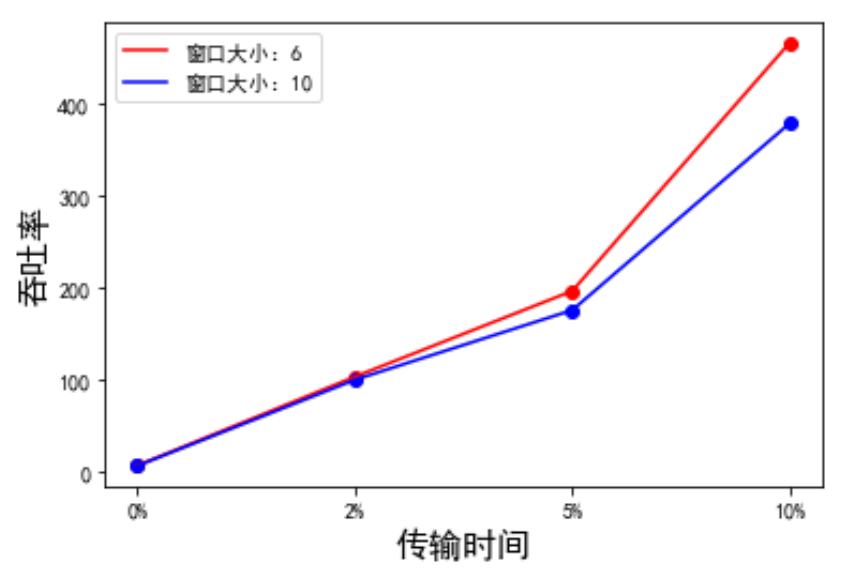
\includegraphics[scale=0.6]{计网6.png}
    \label{fig:6}
\end{figure}
\subsubsection{改变延时}
延时单位为ms。丢包设为0,得到结果如下所示:
表
\begin{table}[!htbp]
  \centering
  \begin{tabular}{ccccccccccc}
  \toprule  
  窗口大小$\backslash$延时& 0s& 20s& 50s& 100s\\
  \midrule
  6& 1022.32& 125.453& 65.6478& 45.2397\\
  10& 1044.26& 126.833& 70.5729& 49.8144\\
  \bottomrule
  \end{tabular}
  \caption{性能测试吞吐率结果(单位:Kbps)}
\end{table}

关于传输时间,由于使用路由程序转发本身就会带来一定的延时,因此这里的数据并不能真实反映程序性能。
\begin{table}[!htbp]
  \centering
  \begin{tabular}{ccccccccccc}
  \toprule  
  窗口大小$\backslash$丢包率& 0\%& 2\%& 5\%& 10\%\\
  \midrule
  6& 6.842& 205.134& 396.136& 702.100\\
  10& 6.391& 188.624& 386.886& 663.311\\
  \bottomrule
  \end{tabular}
  \caption{性能测试延时结果(单位:S)}
\end{table}

绘制曲线如下所示:
\begin{figure}[H]
    \centering
    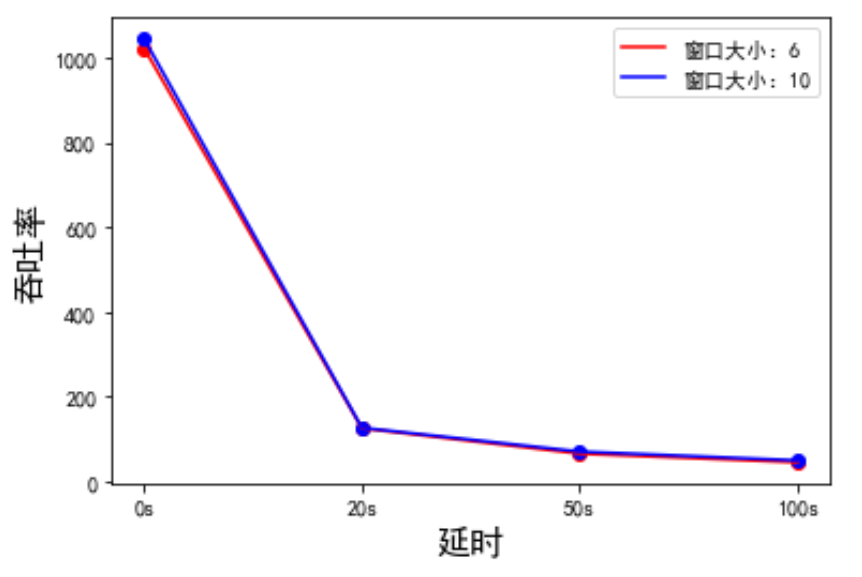
\includegraphics[scale=0.6]{计网7.png}
    \label{fig:7}
\end{figure}
\begin{figure}[H]
    \centering
    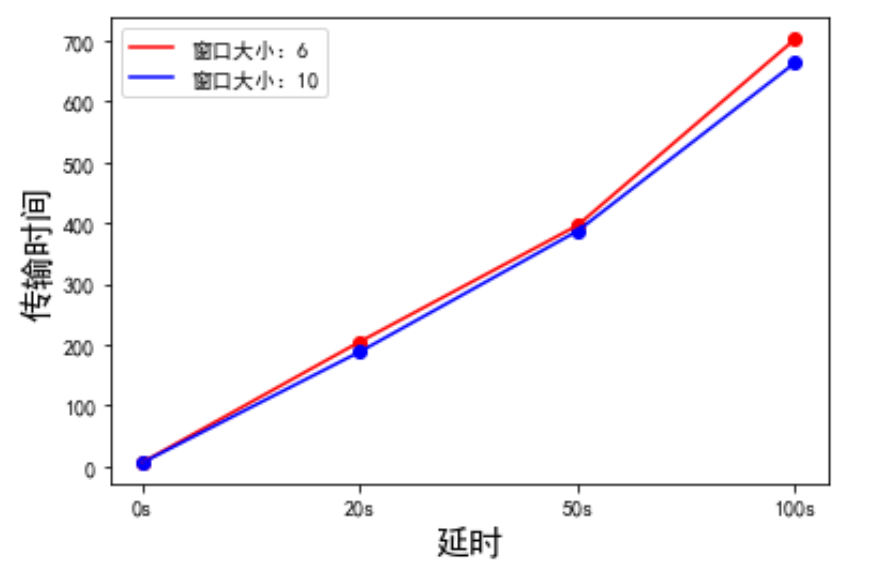
\includegraphics[scale=0.6]{计网8.png}
    \label{fig:8}
\end{figure}
\subsubsection{结果分析}
总体来说:
不同窗口大小在不同网络环境下的效率变化总体上趋于一致\par
在网络情况较好的时候窗口大的效率更高,因为更大的窗口可以允许同时发送更多条消息并同时等待对方的ACK,此时丢包率较小,使用更大的滑动窗口一次能发出更多的包,而没有太多的丢包导致的重传,所以能起到较好的加速效果,即减少等待的周期数,更好的应对时延问题。\par
对于丢包问题,当丢包率较高时由于大的窗口会增加重传代价,使用更大的滑动窗口相对于较小的滑动窗口性能优势明显减弱,甚至在有几次测试中,性能不如更较小滑动窗口。分析重传机制,当有较多丢包时,滑动窗口需要累积确认ACK、重传失序未确认的数据包,当这些失序的数据包ACK收到后才能移动窗口,因此有较多的性能损失。尤其是当路由延时设置较大时,性能损失更明显。
\subsection{有拥塞控制和无拥塞控制的性能比较}
\subsubsection{改变丢包率}
延时设为0,得到结果如下所示:
表
\begin{table}[!htbp]
  \centering
  \begin{tabular}{ccccccccccc}
  \toprule  
  是否有拥塞控制$\backslash$丢包率& 0\%& 2\%& 5\%& 10\%\\
  \midrule
  是& 1300.11& 402.673& 201.129& 80.8068\\
  否& 1044.26& 343.323& 198.482& 69.5384\\
  \bottomrule
  \end{tabular}
  \caption{性能测试吞吐率结果(单位:Kbps)}
\end{table}

关于传输时间,由于使用路由程序转发本身就会带来一定的延时,因此这里的数据并不能真实反映程序性能。
\begin{table}[!htbp]
  \centering
  \begin{tabular}{ccccccccccc}
  \toprule  
  是否有拥塞控制$\backslash$丢包率& 0\%& 2\%& 5\%& 10\%\\
  是& 6.855& 27.288& 59.313& 165.192\\
  否& 6.499& 30.143& 58.667& 195.321\\
  \bottomrule
  \end{tabular}
  \caption{性能测试延时结果(单位:S)}
\end{table}

绘制曲线如下所示:
\begin{figure}[H]
    \centering
    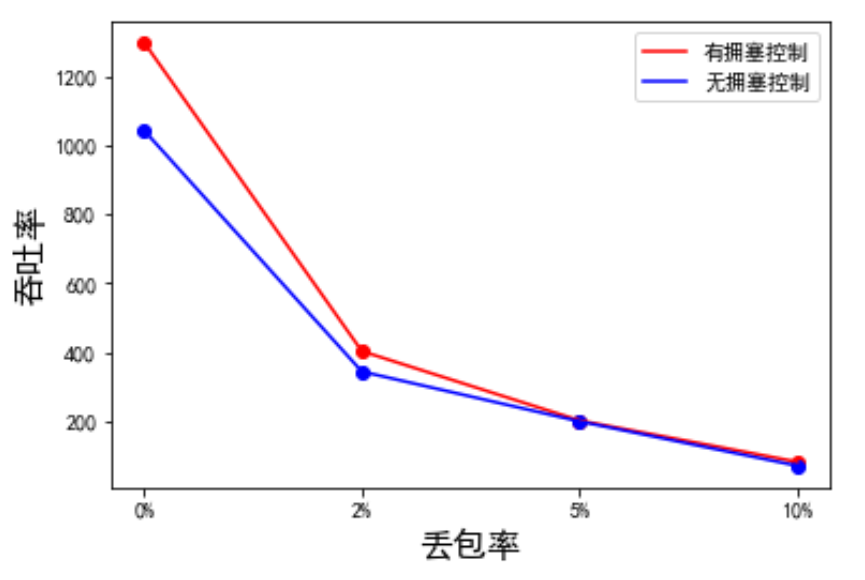
\includegraphics[scale=0.6]{计网9.png}
    \label{fig:9}
\end{figure}
\begin{figure}[H]
    \centering
    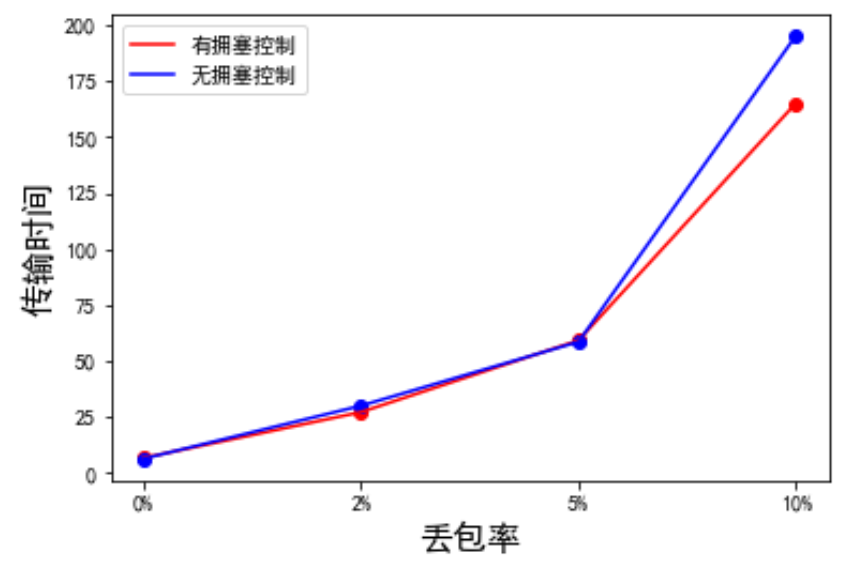
\includegraphics[scale=0.6]{计网10.png}
    \label{fig:10}
\end{figure}
\subsubsection{改变延时}
延时单位为ms。丢包设为0,得到结果如下所示:
表
\begin{table}[!htbp]
  \centering
  \begin{tabular}{ccccccccccc}
  \toprule  
  是否有拥塞控制$\backslash$延时& 0s& 20s& 50s& 100s\\
  \midrule
  是& 1221.178& 509.642& 169.534& 46.711\\
  否& 1044.26& 526.833& 170.572& 49.8144\\
  \bottomrule
  \end{tabular}
  \caption{性能测试结果(4线程)(单位:ms)}
\end{table}

关于传输时间,由于使用路由程序转发本身就会带来一定的延时,因此这里的数据并不能真实反映程序性能。
\begin{table}[!htbp]
  \centering
  \begin{tabular}{ccccccccccc}
  \toprule  
  是否有拥塞控制$\backslash$延时& 0s& 20s& 50s& 100s\\
  是& 7.115& 115.819& 254.331& 355.801\\
  否& 7.030& 109.631& 277.082& 405.293\\
  \bottomrule
  \end{tabular}
  \caption{性能测试延时结果(单位:S)}
\end{table}

绘制曲线如下所示:
\begin{figure}[H]
    \centering
    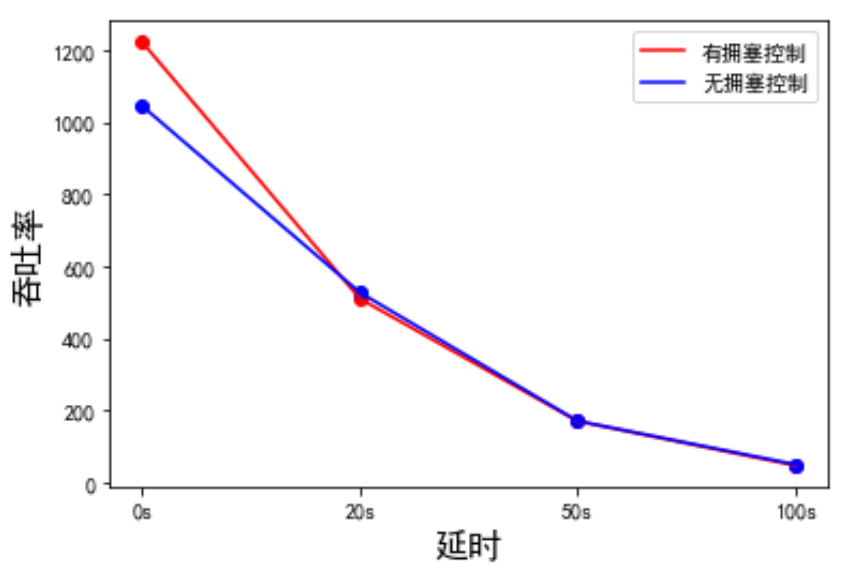
\includegraphics[scale=0.6]{计网11.png}
    \label{fig:11}
\end{figure}
\begin{figure}[H]
    \centering
    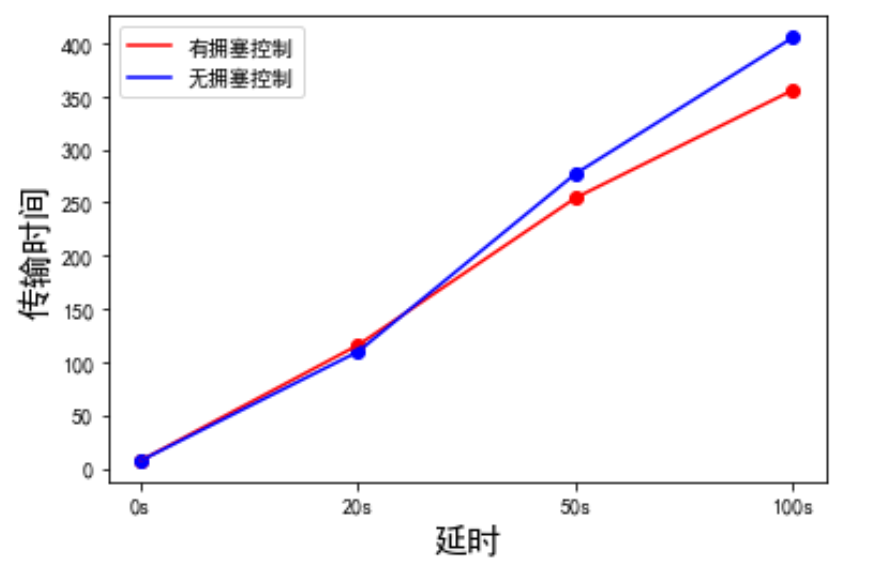
\includegraphics[scale=0.6]{计网12.png}
    \label{fig:12}
\end{figure}
\subsubsection{结果分析}
总体来说:
在网络情况良好时,有拥塞控制相对于没有拥塞控制效率更高,因为拥塞控制可以允许有更大的窗口,快速重传机制也可以减少等待超时重传的次数。\par
当网络情况逐渐变差时,拥塞控制机制表现可能并不比没有拥塞控制好,频繁缩小窗口导致窗口较小,小于没有拥塞控制机制的设定值,导致受时延的影响较大\par
实验过程中也发现,当网络情况变得更差时,拥塞控制机制可能使窗口由几百突然降至1,并进入重传,使得重传代价飞速增加。
\section{总结与一些问题}
整体来说,本次实验较为成功。合理地对比了不同的协议和设计之间的性能差异,使我对计算机网络的内容有了更加深入的认识。同时,由于实验采用router.exe,感觉这个路由程序本身对实验所得到的数据影响较大。最后,网络的稳定也是实验顺利进行的关键。在网络有波动的时候,同样的变量可能会呈现出相反的结论,这也是需要注意的。
\end{document}